%===================================== CHAP 5 =================================

\chapter{Experiments and Results}

\section{Introduction}

Chapter 3 discuss the different concepts regarding the pipeline and the examples data managed by it. Chapter 4 explains how the pipeline is implemented. In this chapter we will use the information made available in Chapter 3 and 4 and explore to what degree the research goals have been accomplished. First, for Research Goal 1 we will decide whether the pipeline created is satisfactory or not. Regarding Research Goal 2, we will conclude the analysis conducted in Chapter 3. Next, we will investigate if the database chosen to manage the collection of examples, is satisfying the purpose of Research Goal 3. Finally, a series of tests will be performed to measure the search results displayed by the search interface. A comparison of the results will help determine if Research Goal 4 is fulfilled.

\section{Pipeline}

We tested the final pipeline by using the English Wikipedia's database dump from February 4. 2016. With a size of 56.3 GB, the XML file contains over five million articles. The process of extracting the relevant data and inserting it into the SQL database, lasted nine hours. After the last section was added, the database contained 28 110 sections deemed as relevant sections.

When the process that extract relevant sections were finished, a new fully independent process was started for the next step. To begin with, the process queries the SQL database for sections. By using the relations from the sections stored in the SQL database, the process builds examples. Next, a white list is used to filter the examples based on their categories. By filtering the examples we can avoid uninteresting categories, for instance examples concerning history. Finally, the collection of examples left are used to build an index with Elasticsearch. The Elasticsearch index offers a HTTP API that other processes can use to query for examples.

\begin{table}[h!]
\centering
\begin{tabular} {|| p{15em} | r ||} 
 \hline
  & Value \\ [0.5ex] 
 \hline
XML file size in Gigabytes & 56.3 \\
Number of articles & ~5 100 000 \\
Extraction duration in hours & ~9 \\
Number of section after extraction & 28110 \\
Number of examples after filtering & 6593 \\

 \hline
\end{tabular}
\caption{Statistics from a run through the pipeline}
\label{table:run_statistics}
\end{table}


\section{Finding a good example}
Finding examples is the overall goal of this work, in order to use the system we have created. Without useful data, the system is worthless. Therefore we want to fill our database with good examples. This project use Wikipedia as a source to automatically identify and extract examples. To make the best out of the examples extracted, we performed an analysis on what differentiates a good example from a bad one. A more detailed account of the analysis can be found in section \ref{examples-section}. This section will use the main points from section \ref{examples-section} to draw a conclusion.

The analysis was performed based on examples from Wikipedia, but to compare examples for the same subject, examples from other sources were also used. Game Theory is used as an overall domain for the analysis. The following subjects were chosen to find examples about, Prisoners Dilemma, Nash Equilibrium, Pareto Optimality, Zero sum, Parrondos Paradox. Appendix \ref{app_example} contains samples of two examples chosen for the subject Pareto Optimality. 

Based on these samples, a list of properties that examples might possess was compiled, table \ref{table:1} contains these properties with a short description of each. The properties listed in table \ref{table:1} are all favourable, but we experienced that when an example contains to many of them, it becomes very complex. A complex example is not necessarily a bad thing. Although a more complex example requires more prerequisite knowledge from the reader, which may exclude some readers. The extent of use for each property is also a considerable factor for determining complexity. Although more properties often add more complexity, some are always needed. A simple example will have a hard time explaining the more complicated aspects of a subject. Therefor an example should fall in between a golden mean of complexity. This golden mean is hard to define, but ought to be quite large. There is some techniques though, that lets an example explain more complicated subjects, without increasing complexity. Pictures or equations that is methodically referenced to from a descriptive text, is one way. Also the combination of the properties analogies, walk-through and iterations improve examples without making them more complex. 

The analysis in section \ref{examples-section} gave a better understanding of examples. Consequently rating and ordering of examples can be improved based on the analysis. 
The improvement can result in the collection of examples having a higher quality and also lead to a better user experience. 


\section{Collection of examples}
Reaserch Goal 3 aims to obtain a collection of examples that we can populate a database with. The database accepts all kinds of examples, consequently the examples are represented in a generic way. We are using Wikipedia as source for all the examples, therefor we have to strip away a large amount of the information from the articles used. 

After an article is extracted from the XML document, data is stored in a relational database. To form an example, data is fetched from the tables by using the relations defined in the SQL database. In addition to the content, categories and references associated with the example are included. These properties are needed for an example in our system, so we later can perform queries on the collection. With Wikipedia having no limits for its domains, white lists are used to narrow the examples down into only relevant domains for our project.

After the processing, the collection now contains relevant elements, with a structure that represents a general example. This collection can then be indexed by Elasticsearch, which is the database containing all examples. Other examples from different sources can separately be included to Elasticsearch's example index, as long as the examples are structured correctly according to the mapping described in section \ref{imp_indexer}.


\section{Experiment I: Search examples} \label{search_experiment}
In this project we have filled a database with examples, indexed those examples and created a interface that we can use for searching them. In order to perform searches, we have created queries that Elasticsearch executes. To test how well these queries perform we have created a list of keywords. We test the accuracy of the queries by measuring the precision of the results returned from a search with the selected  keywords. Precision is the fraction of returned examples, which is relevant. It is calculated in this way, \(\frac{|R \cap E |}{|E|}\), where \(R\) is all relevant examples and \(E\) is all the retrieved examples. Precision is often used in combination with Recall, which is the fraction of relevant examples retrieved. Since we do not know how many relevant examples exist in total for each keyword, we can not measure recall. 


\begin{table}[h!]
\centering
\begin{tabular} {|| p{15em} | r | r | r ||} 
 \hline
 Keyword & Total hits & Top 5 & Top 10 \\ [0.5ex] 
 \hline

Logic & 362 & 1 & 0.9 \\
Programming & 884 & 1 & 0.9 \\
Heuristic & 44 & 0.8 & 0.7 \\
Algebra & 1046 & 0.8 & 0.7 \\
Game Theory & 2757 & 1 & 0.9 \\
\hline
Fuzzy Logic & 365 & 1 & 0.7 \\
Java & 269 & 1 & 0.9 \\
Bayes Network & 345 & 1 & 0.9 \\
Derivation & 67 & 1 & 0.8 \\
\hline
Chain Rule & 530 & 1 & 0.6 \\
Prisoners Dilemma & 39 & 1 & 0.6 \\
Nash Equilibrium & 101 & 1 & 0.8 \\
Cartesian Product & 789 & 0.8 & 0.6 \\
Parrondos Paradox & 49 & 0.6 & 0.4 \\
Zero Sum & 1017 & 0 & 0 \\

 \hline
\end{tabular}
\caption{The precision of the queries tested by a set of keywords and the top ten and top five results}
\label{table:precision_test}
\end{table}

Table \ref{table:precision_test} contains the keywords and the results of the test. The keywords were chosen from the domains mathematics, artificial intelligence and programming. Results returned that simply is not a working example or is an example for another subject is judged as an irrelevant result. Total hits reflects the amount of examples that the program found relevant to any degree. The different keywords have been divided into three different groups. The groups are ordered descending by the degree of how general the keyword is perceived. The horizontal line in the table separates the groups. There is no specific order among the keywords within a group.

At the top of the list the score for five and ten terms are very similar, while towards the bottom where the subjects are more specific, the score for top ten results suffers. Having a relatively small database of examples for specific subjects is assumed to be the explanation.

Another interesting remark to note is that the top 5 results are consistently better than the top 10 results. Top 5 being better than top 10, is caused by at least half of the relevant examples which is returned, are found among the first five results. Therefor we can conclude that the ranking of the examples functions as intended. 

There exist one substantial irregularity in table \ref{table:precision_test} though, the keyword \textit{Zero Sum} achieves a score of zero on both measures, meaning all of the ten first results returned is deemed irrelevant. No relevant results among the first ten could indicate an error in the system, either in the search itself, or that there is no example to find at all. Whether the case is an error in the system or that the keyword is an search term the system handles poorly will be investigated.

While performing the experiment, the error occurred when searching with the keyword \textit{zero sum}. The system should have returned the example section from Wikipedia's article, \textit{Zero-sum game} \footnote{\url{https://en.wikipedia.org/wiki/Zero-sum\_game\#Example}(Last visited 28. April 2016)}. An error analysis will help determine where in the system an error could have originated. 

To find the potential error we start at the beginning of the pipeline, to explore whether the example is retrieved from the XML dump. We find the answer in the SQL database. First we find a row in the \texttt{pages} table with the name \textit{zero sum game}. Next, using the primary key of this row, we can find all related rows in the table \texttt{page\_sections}. A query on the column \texttt{page\_id} in \texttt{page\_sections} returns one result. This result is the same section found in Wikipedia's article, thus we can conclude that Wikidump parser successfully inserts the section into the SQL database.

The next step is to verify that the section is transformed to an example and indexed by Elasticsearch. The examples in Elasticsearch shares the same id as the sections primary key in the SQL database. Querying Elasticsearch by id returns no results, therefor we know that the zero sum example never reaches Elasticsearch. Between the SQL database and Elasticsearch a white list filters the examples. If the zero-sum game article does not contain a category that exists in the white list, the example will be discarded. The article contains the categories \textit{Non-cooperative games} and \textit{International relations theory}. Matching the article's categories with the complete category list reveals that there exist only 4 occurrences of articles with Non-cooperative games as category and 7 with International relations theory, which is a low number. White list Top200Edu and MathTechWiki were used for the filtering, section \ref{imp_indexer} explains white list's implementation and their function in our project. Top200Edu includes only the top 200 relevant articles and MathTechWiki use only the top level categories in the Wikipedia's category hierarchy. In conclusion, the article's categories is not included in any of the white lists, and therefor the example is not indexed.

If the article's list of categories had been richer, the example would have been included more likely. Although richer category lists for Wikipedia's articles would have solved the problem, it is not something our project can affect. Instead a white list that accommodates the less popular categories is a better solution. The problem is that all the categories have to be manually added to white lists. The White list Edu deals with the problem by including all categories, but also examining the most popular and removing the irrelevant categories from the white list. The disadvantage obtained by using Edu is that irrelevant categories will be included, but on the other hand, they are not connected to many articles. 

\section{Experiment II: White list}

The result of the error analysis in section \ref{search_experiment} points out the significance of the white lists used for the end result. Based on that, Experiment II will be conducted to explore to what the degree the white lists affect the results returned, and which of them is best to use. The tables used to display the result, will be identical to table \ref{table:precision_test} used in section \ref{search_experiment} with one exception. The tables in this section also includes the percentage of hits compared to the number of examples in the index, when each specific white list has been applied. 

The first step in the experiment is to check what the system returns when there is no white lists used. When no white lists are used, there exists 28 110 examples in the index. Table \ref{table:p_test_no-list} shows the results.

\begin{table}[H]
\centering
\begin{tabular} {|| p{10em} | r | r | r | r ||} 
 \hline
 Keyword & Total hits & \% of hits & Top 5 & Top 10 \\ [0.5ex] 
 \hline

Logic & 898 & 3.19 & 1 & 1 \\
Programming & 2135 & 7.60 & 0.8 & 0.9 \\
Heuristic & 81 & 0.29 & 1 & 0.8 \\
Algebra & 1629 & 5.80 & 1 & 0.9 \\
Game Theory & 6301 & 22.42 & 0.8 & 0.9 \\
\hline
Fuzzy Logic & 913 & 3.25 & 1 & 0.7 \\
Java & 523 & 1.86 & 0.8 & 0.9 \\
Bayes Network & 1370 & 4.87 & 0.8 & 0.9 \\
Derivation & 178 & 0.63 & 0.6 & 0.5 \\
\hline
Chain Rule & 1760 & 6.26 & 0.8 & 0.6 \\
Prisoners Dilemma & 141 & 0.50 & 0.8 & 0.5 \\
Nash Equilibrium & 350 & 1.25 & 1 & 1 \\
Cartesian Product & 2119 & 7.54 & 0.6 & 0.7 \\
Parrondos Paradox & 159 & 0.57 &  0.2 & 0.2 \\
Zero Sum & 2330 & 8.29 & 0 & 0.1 \\

 \hline
\end{tabular}
\caption{The precision of the queries tested when all examples are included.}
\label{table:p_test_no-list}
\end{table}

In the next step white list Edu will be tested. Edu contains most of the categories from the orignal category list, with the exception of categories that are popular, but not educational, being removed. A category's popularity is measured in how many examples links to the category. When the examples are filtered through Edu, 5 133 examples are discarded from the original 28 110. The results of the test can be found in table \ref{table:p_test_list1}.

%%whitelist 1 : filtrert 5133 av 28110
\begin{table}[H]
\centering
\begin{tabular} {|| p{10em} | r | r | r | r ||} 
 \hline
 Keyword & Total hits & \% of hits & Top 5 & Top 10 \\ [0.5ex] 
 \hline

Logic & 737 & 3.21 & 1 & 1 \\
Programming & 1783 & 7.76 & 0.8 & 0.9 \\
Heuristic & 72 & 0.31 & 1 & 0.8 \\
Algebra & 1337 & 5.82 & 1 & 0.8 \\
Game Theory & 5230 & 22.76 & 0.8 & 0.9 \\
\hline
Fuzzy Logic & 750 & 3.26 & 1 & 0.8 \\
Java & 442 & 1.92 & 0.8 & 0.9 \\
Bayes Network & 1171 & 5.10 & 0.8 & 0.9 \\
Derivation & 145 & 0.63 & 0.4 & 0.5 \\
\hline
Chain Rule & 1374 & 5.98 & 0.8 & 0.6 \\
Prisoners Dilemma & 115 & 0.50 & 0.8 & 0.5 \\
Nash Equilibrium & 60 & 0.26 & 1 & 1 \\
Cartesian Product & 1739 & 7.57 & 0.6 & 0.6 \\
Parrondos Paradox & 128 & 0.56 & 0.2 & 0.2 \\
Zero Sum & 1842 & 8.02 & 0 & 0.1 \\

 \hline
\end{tabular}
\caption{The precision of the queries tested when white list Edu is used to filter the collection beforehand}
\label{table:p_test_list1}
\end{table}

The third test is conducted on white list Top200Edu. Top200Edu is similar to Edu in terms of what type of categories are removed from the original list, with one big difference. Top200Edu only keeps the 200 most popular categories, which means the educational categories which are not popular enough, are not included. Using Top200Edu results in 21 746 examples being excluded from the index. Table \ref{table:p_test_list2} displays the results.

%%whitelist 2 : filtrert 21746 av 28110
\begin{table}[H]
\centering
\begin{tabular} {|| p{10em} | r | r | r | r ||} 
 \hline
 Keyword & Total hits & \% of hits & Top 5 & Top 10 \\ [0.5ex] 
 \hline

Logic & 338 & 5.31 & 1 & 0.9 \\
Programming & 864 & 13.58 & 0.8 & 0.9 \\
Heuristic & 31 & 0.49 & 1 & 0.5 \\
Algebra & 1034 & 16.25 & 1 & 1 \\
Game Theory & 2701 & 42.44 & 0.8 & 0.8 \\
\hline
Fuzzy Logic & 341 & 5.36 & 0.8 & 0.5 \\
Java & 267 & 4.20 & 1 & 1 \\
Bayes Network & 315 & 4.96 & 1 & 0.9 \\
Derivation & 62 & 0.97 & 1 & 0.9 \\
\hline
Chain Rule & 515 & 8.09 & 1 & 0.6 \\
Prisoners Dilemma & 38 & 0.60 & 0.8 & 0.5 \\
Nash Equilibrium & 100 & 1.57 & 1 & 1 \\
Cartesian Product & 748 & 11.75 & 0.6 & 0.6 \\
Parrondos Paradox & 46 & 0.72 & 0.4 & 0.4 \\
Zero Sum & 1842 & 28.94 & 0 & 0 \\

 \hline
\end{tabular}
\caption{The precision of the queries tested when white list Top200Edu is used to filter the collection beforehand}
\label{table:p_test_list2}
\end{table}

In the fourth step, we test white list MathTech. MathTech is based on Top200Edu, but it narrows the domains of the categories deemed relevant to only concern Technology and Mathematics. MathTech is a bit smaller than Top200Edu, with 157 different categories. 23 073 examples are filtered out, when MathTech is used. Table \ref{table:p_test_list3} reflects the results of the test.

%%whitelist 3: filtrert 23073 av 28110
\begin{table}[H]
\centering
\begin{tabular} {|| p{10em} | r | r | r | r ||} 
 \hline
 Keyword & Total hits & \% of hits & Top 5 & Top 10 \\ [0.5ex] 
 \hline

Logic & 326 & 6.47 & 1 & 0.9 \\
Programming & 852 & 16.91 & 0.8 & 0.9 \\
Heuristic & 19 & 0.38 & 0.8 & 0.6 \\
Algebra & 991 & 19.67 & 1 & 1 \\
Game Theory & 2386 & 47.37 & 0.8 & 0.9 \\
\hline
Fuzzy Logic & 329 & 6.53 & 0.8 & 0.5 \\
Java & 265 & 5.26 & 1 & 1 \\
Bayes Network & 262 & 5.20 & 1 & 0.9 \\
Derivation & 56 & 1.11 & 1 & 1 \\
\hline
Chain Rule & 402 & 7.98 & 1 & 0.6 \\
Prisoners Dilemma & 33 & 0.66 & 0.8 & 0.5 \\
Nash Equilibrium & 87 & 1.73 & 1 & 1 \\
Cartesian Product & 606 & 12.03 & 0.6 & 0.6 \\
Parrondos Paradox & 37 & .73 & 0.4 & 0.4 \\
Zero Sum & 917 & 18.21 & 0 & 0 \\

 \hline
\end{tabular}
\caption{The precision of the queries tested when white list MathTech is used to filter the collection beforehand}
\label{table:p_test_list3}
\end{table}

In the final step we test the most conservative white list, MathTechWiki. MathTechWiki is based on Wikipedia's category hierarchy, were Mathemathics, Logic, Mathematical Sciences, Computing and their sub categories have been included. Applying MathTechWiki leads to the removal of 27 107 examples. Table \ref{table:p_test_list4} contains the results of the final test. 

%%whitelist 4: filtrert 27107 av 28110
\begin{table}[H]
\centering
\begin{tabular} {|| p{10em} | r | r | r | r ||} 
 \hline
 Keyword & Total hits & \% of hits & Top 5 & Top 10 \\ [0.5ex] 
 \hline

Logic & 100 & 9.97 & 1 & 1 \\
Programming & 107 & 10.67 & 0.2 & 0.3 \\
Heuristic & 20 & 1.99 & 0.6 & 0.4 \\
Algebra & 165 & 16.45 & 0.8 & 0.6 \\
Game Theory & 476 & 47.46 & 0.8 & 0.8 \\
\hline
Fuzzy Logic & 101 & 10.07 & 1 & 0.6 \\
Java & 9 & 0.90 & 0.4 & 3/9 \\
Bayes Network & 102 & 10.17 & 0.8 & 0.6 \\
Derivation & 22 & 2.19 & 0.6 & 0.4 \\
\hline
Chain Rule & 120 & 11.96 & 0.2 & 0.1 \\
Prisoners Dilemma & 8 & 0.80 & 0.4 & 2/8 \\
Nash Equilibrium & 17 & 1.69 & 1 & 0.9 \\
Cartesian Product & 126 & 12.56 & 0 & 0.1 \\
Parrondos Paradox & 18 & 1.79 & 0 & 0 \\
Zero Sum & 169 & 16.85 & 0.2 & 0.1 \\

 \hline
\end{tabular}
\caption{The precision of the queries tested when white list MathTechWiki is used to filter the collection beforehand}
\label{table:p_test_list4}
\end{table}




\begin{figure}[h] 
\caption{Precision score when the keyword \textit{Logic} is used as a search phrase, with the different white lists applied.}
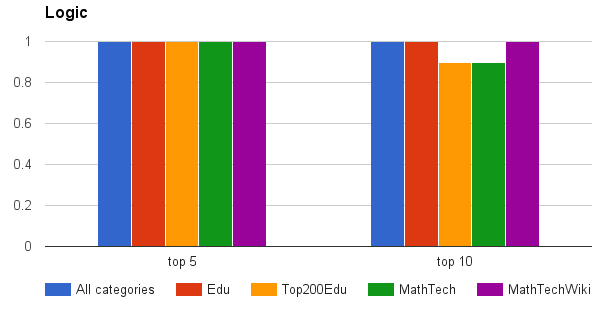
\includegraphics[width=\textwidth]{charts/l}
\label{fig:l}
\end{figure}

\begin{figure}[h] 
\caption{Precision score when the keyword \textit{Programming} is used as a search phrase, with the different white lists applied.}
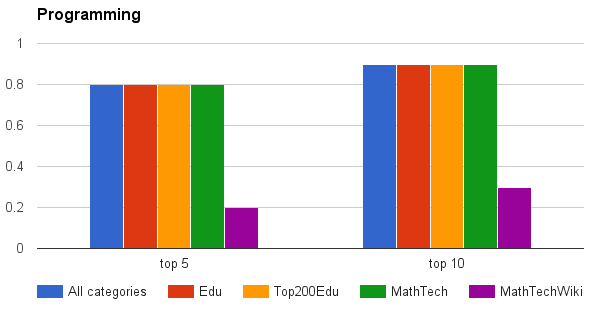
\includegraphics[width=\textwidth]{charts/p}
\label{fig:p}
\end{figure}

\begin{figure}[h] 
\caption{Precision score when the keyword \textit{Heuristic} is used as a search phrase, with the different white lists applied.}
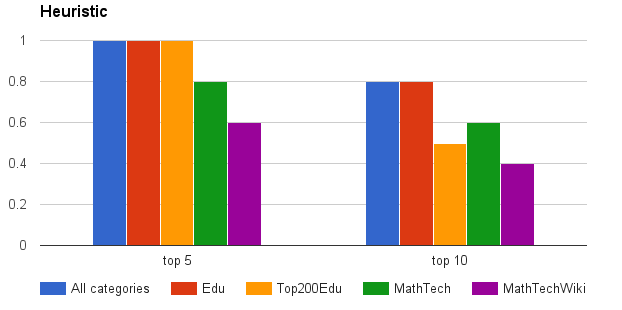
\includegraphics[width=\textwidth]{charts/h}
\label{fig:h}
\end{figure}

\begin{figure}[h] 
\caption{Precision score when the keyword \textit{Algebra} is used as a search phrase, with the different white lists applied.}
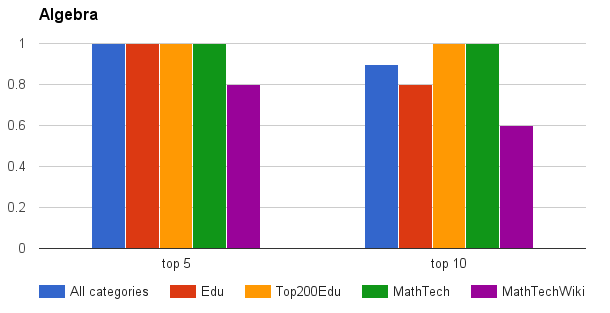
\includegraphics[width=\textwidth]{charts/a}
\label{fig:a}
\end{figure}

\begin{figure}[h] 
\caption{Precision score when the keyword \textit{Game Theory} is used as a search phrase, with the different white lists applied.}
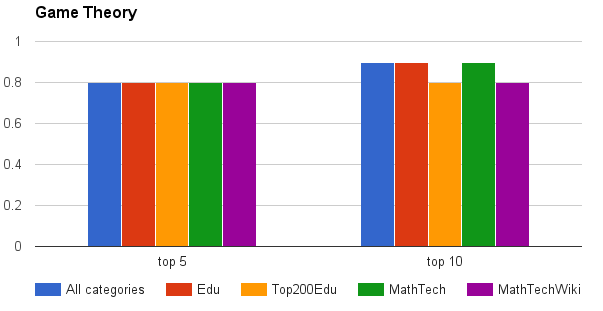
\includegraphics[width=\textwidth]{charts/gt}
\label{fig:gt}
\end{figure}

\begin{figure}[h] 
\caption{Precision score when the keyword \textit{Fuzzy Logic} is used as a search phrase, with the different white lists applied.}
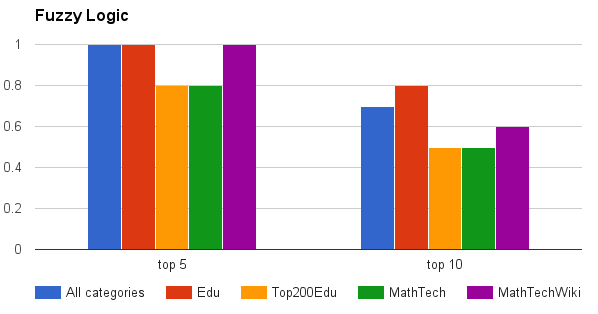
\includegraphics[width=\textwidth]{charts/fl}
\label{fig:fl}
\end{figure}



\begin{figure}[h] 
\caption{Precision score when the keyword \textit{Bayes Network} is used as a search phrase, with the different white lists applied.}
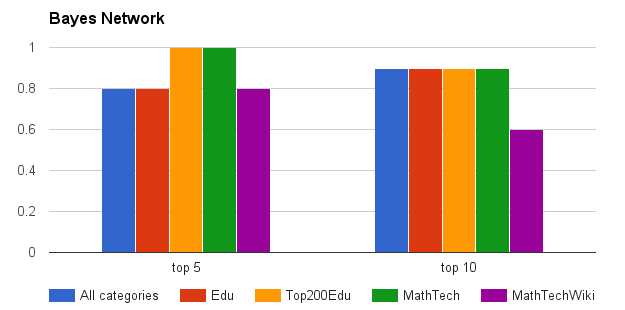
\includegraphics[width=\textwidth]{charts/bn}
\label{fig:bn}
\end{figure}



\begin{figure}[h] 
\caption{Precision score when the keyword \textit{Chain Rule} is used as a search phrase, with the different white lists applied.}
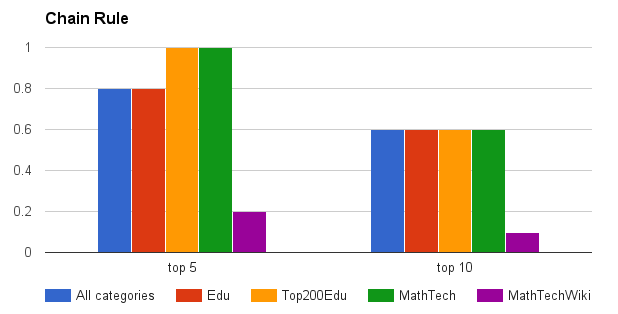
\includegraphics[width=\textwidth]{charts/cr}
\label{fig:cr}
\end{figure}

\begin{figure}[h] 
\caption{Precision score when the keyword \textit{Prisoners Dilemma} is used as a search phrase, with the different white lists applied.}
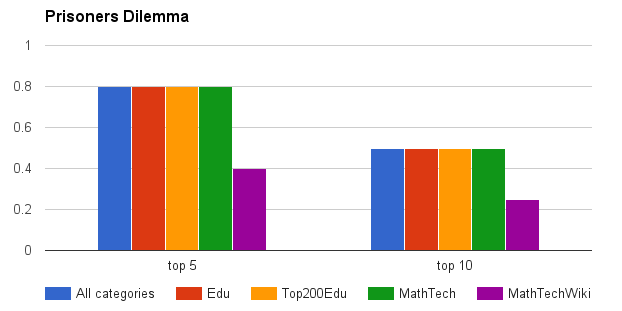
\includegraphics[width=\textwidth]{charts/pd}
\label{fig:pd}
\end{figure}

\begin{figure}[h] 
\caption{Precision score when the keyword \textit{Nash Equilibrium} is used as a search phrase, with the different white lists applied.}
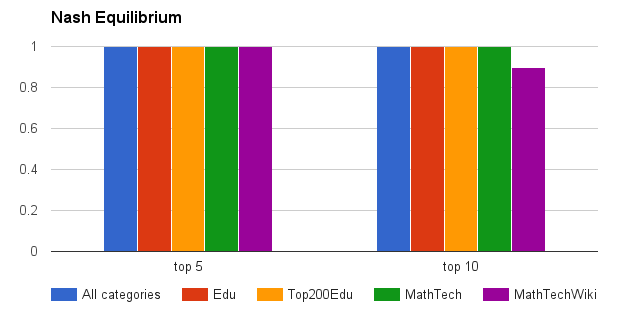
\includegraphics[width=\textwidth]{charts/ne}
\label{fig:ne}
\end{figure}

\begin{figure}[h] 
\caption{Precision score when the keyword \textit{Cartesian Product} is used as a search phrase, with the different white lists applied.}
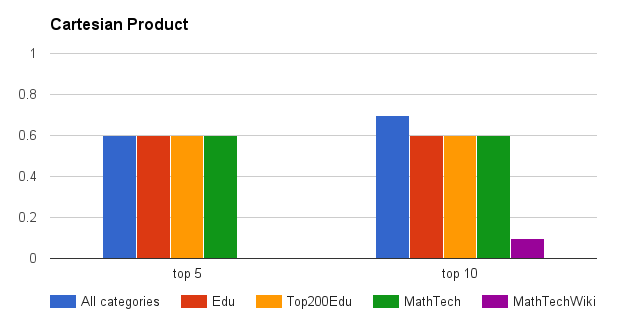
\includegraphics[width=\textwidth]{charts/cp}
\label{fig:cp}
\end{figure}

\begin{figure}[h] 
\caption{Precision score when the keyword \textit{Parrondos Paradox} is used as a search phrase, with the different white lists applied.}
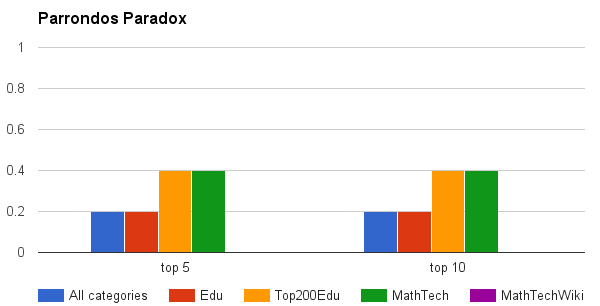
\includegraphics[width=\textwidth]{charts/pp}
\label{fig:pp}
\end{figure}







\cleardoublepage